\documentclass[fleqn, 10pt]{article}

% Paquetes necesarios
\usepackage[utf8]{inputenc}
\usepackage[english]{babel}
\usepackage{amsthm, amsmath}
\usepackage{nccmath} %Para centrar ecuaciones
\usepackage{graphicx}
\graphicspath{ {Documentos/} }
\usepackage{tikz}
\usetikzlibrary{automata,arrows.meta,positioning}


% Personalizo mi alfabeto
\DeclareMathAlphabet{\pazocal}{OMS}{zplm}{m}{n}
\newcommand{\Lb}{\pazocal{L}}

% Definimos los entornos para definiciones, teoremas, etc...
\theoremstyle{plain}
\newtheorem{proposicion}{Proposición}

\theoremstyle{definition}
\newtheorem{definition}{Definición}[section]
\newtheorem{example}{Ejemplo}[section]

%Definimos el título
\title{Teoría de Autómatas y Lenguajes Formales\\[.4\baselineskip]Práctica 2}
\author{Irene, Recio López}
\date{\today}

%Comienzo del documento
\begin{document}

%Generamos el título
\maketitle

\subsubsection*{Ejercicio 1 y 2: Crear un DFA que siendo el alfabeto {a,b}, el lenguaje solo reconoce a la cadena "a" y hacerlo y comprobarlo tambien en OCTAVE}
\begin{center}
Let $M=(\{q_0,q_1,q_2\}, \{a,b\}, \delta, q_0, \{q_1\})$ be a DFA with:\\

\begin{table}[h!]
\begin{tabular}{c|c|c}
 $\delta(q,\sigma)$ & $a$ & $b$
\\
 \hline
 $q_0$& $q_1$ & $q_2$\\
  \hline
  $q_1$& $q_2$ & $q_2$\\
  \hline
  $q_2$& $q_2$ & $q_2$
\end{tabular}
\end{table} 
\end{center}
Automata diseñado con JFLAP
\\
	\centering
	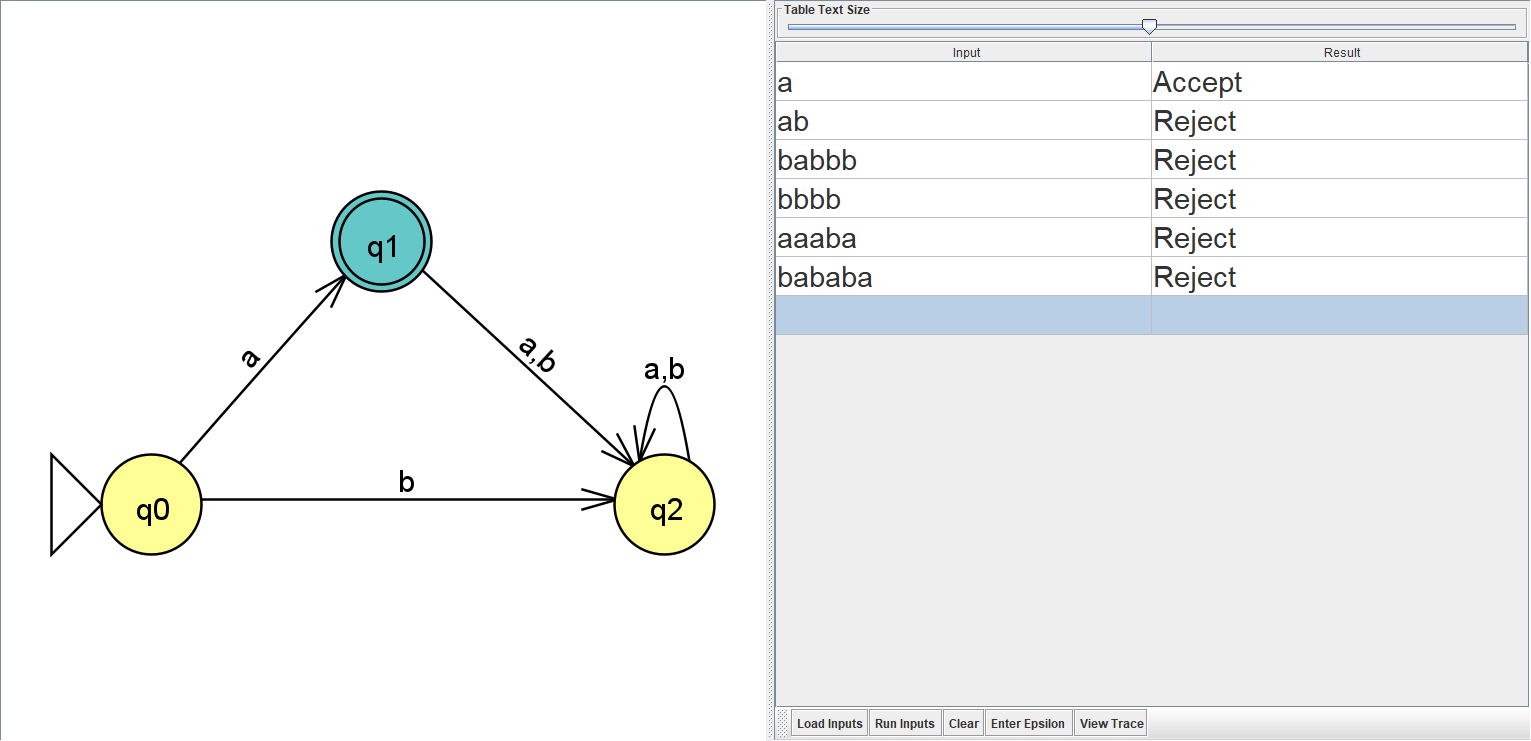
\includegraphics[scale=0.2]{resultados}

\begin{flushleft}
Creo el autómata en el archivo finiteautomata.json:



\end{flushleft}
\begin{verbatim}
{
    "name" : "a",
    "representation" : {
      "K" : ["q0", "q1", "q2"],
      "A" : ["a", "b"],
      "s" : "q0",
      "F" : ["q1"],
      "t" : [["q0", "a", "q1"],
             ["q0", "b", "q2"],
             ["q1", "a", "q2"],
             ["q1", "b", "q2"],
             ["q2", "a", "q2"],
             ["q2", "b", "q2"]]
      }
  }
\end{verbatim}

\begin{flushleft}
Al ejecutarlo en Octave siguiendo este modelo de automata con la siguiente instrucción:
	\begin{center}
	finiteautomaton("a", "a")
	\end{center}
El automata dado como resultado es el siguiente:

M = ({q0, q1, q2}, {a, b}, {(q0, a, q1), (q0, b, q2), (q1, a, q2), (q1, b, q2), 
\\(q2, a, q2), (q2, b, q2)}, q0, {q1})
\\w = a

$(q_0,a)\vdash(q_1,\epsilon)$

$x \in\Lb(M) $

ans = 1
\end{flushleft}
\end{document}

